\documentclass[thesis.tex]{subfiles}
\begin{document}

\chapter{Object detection}
\label{sec:od}

\section{Sliding window}

$\sigma \cdot 134x70$ (128x64 + 3 pixel border)

\section{Support vector machine}

LIBLINEAR v. 1.94 \cite{fan2008liblinear}


\section{Performance measures}

\section{Dataset}
\label{sec:odDataset}

INRIA Person Dataset \footnote{\url{http://pascal.inrialpes.fr/data/human/}} \cite{dalal2005histograms}

Notes: Pedestrians, somewhat upright persons, all images flipped horizontally.
1218 negative training, 2416 positive train, 1126 positive test, 453 negative test images (320x240,640x480)

\begin{figure}
	\centering
	\begin{subfigure}[t]{\textwidth}
		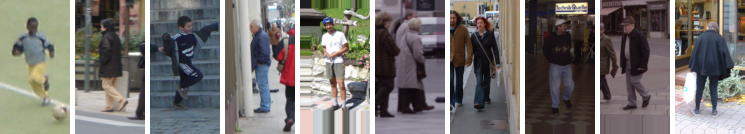
\includegraphics[width=\textwidth]{img/inriaPositives.png}
		\caption{Positives}
		\label{fig:inriaPositives}
		\vspace{2mm}
	\end{subfigure}
	\begin{subfigure}[t]{\textwidth}
		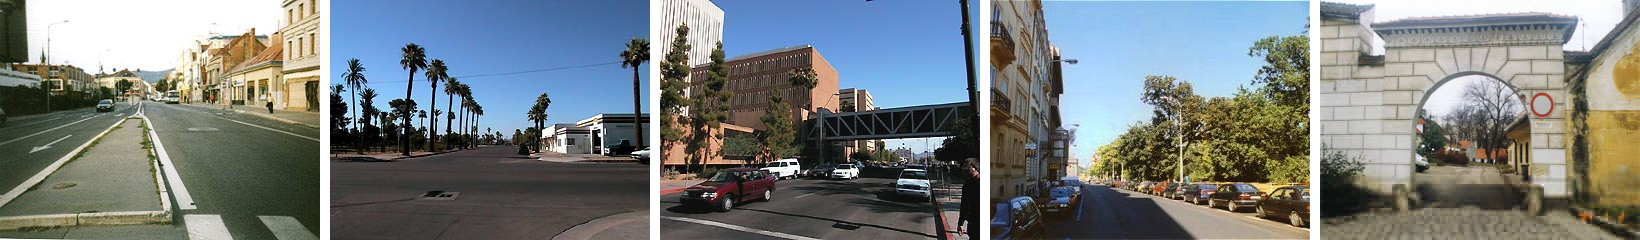
\includegraphics[width=\textwidth]{img/inriaNegatives.png}
		\caption{Negatives}
		\label{fig:inriaNegatives}
	\end{subfigure}
	\caption{Example INRIA images.}
	\label{fig:inriaExampleImages}
\end{figure}

\subsection{Deficiencies 6 pitfalls}
10 duplicate negative train images

\section{Example}

\begin{figure}
	\centering
	\begin{subfigure}[t]{\textwidth}
		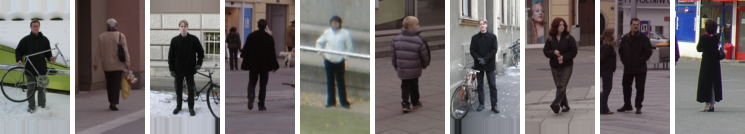
\includegraphics[width=\textwidth]{img/objectDetectionTP.png}
		\caption{True positives}
		\label{fig:objectDetectionTP}
		\vspace{2mm}
	\end{subfigure}
	\begin{subfigure}[t]{\textwidth}
		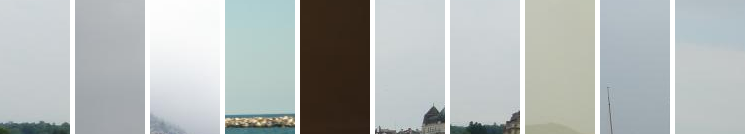
\includegraphics[width=\textwidth]{img/objectDetectionTN.png}
		\caption{True negatives}
		\label{fig:objectDetectionTN}
		\vspace{2mm}
	\end{subfigure}
	\begin{subfigure}[t]{\textwidth}
		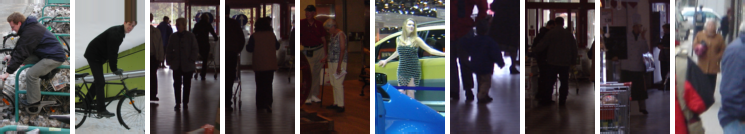
\includegraphics[width=\textwidth]{img/objectDetectionFN.png}
		\caption{False negatives}
		\label{fig:objectDetectionFN}
		\vspace{2mm}
	\end{subfigure}
	\begin{subfigure}[t]{\textwidth}
		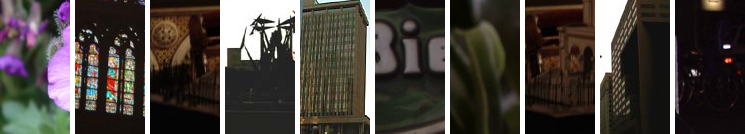
\includegraphics[width=\textwidth]{img/objectDetectionFP.png}
		\caption{False positives}
		\label{fig:objectDetectionFP}
	\end{subfigure}
	\caption{Example classifications of INRIA windows.}
	\label{fig:imageCorrespondenceCurves}
\end{figure}

\section{Parameter study}
\label{sec:odParameterStudy}

\subbibliography

\end{document}
